\chapter{Analýza a~návrh řešení}\label{kap:analyza}
% Analýza a~návrh implementace (včetně diskuse různých alternativ a~volby implementačního prostředí).

% Architektura
%   pocatecni navrh
%   novy navrh: klient - server
%   telnet
%   diskuze nad nacitanim a ukladanim
%   Smerovani + RT (stary navrh - 1 spolecna, novy navrh - wrapper) + prijem paketu
%   NAT 
% Podobnost simulátoru
% Předpokládaný rozsah
% Programovací jazyk
% Paměťová náročnost
% Uživatelské rozhraní

%------------------------------------------------------------------------------

\section{Architektura}

\subsection{Naivní návrh}
Po zadání projektu jsem vytvořil počáteční návrh aplikace a po konzultaci s~kolegou (každý si udělal svůj návrh) vznikl tzv. naivní návrh (viz obrázek \ref{fig:navrh}). Tato prvotní varianta počítala s~připojením do skutečné sítě, ale byla zavržena zejména kvůli složitosti takového systému a časové náročnosti implementace. Navíc propojení s reálnou síť není mezi požadavky.

\begin{figure}[h]
\begin{center}
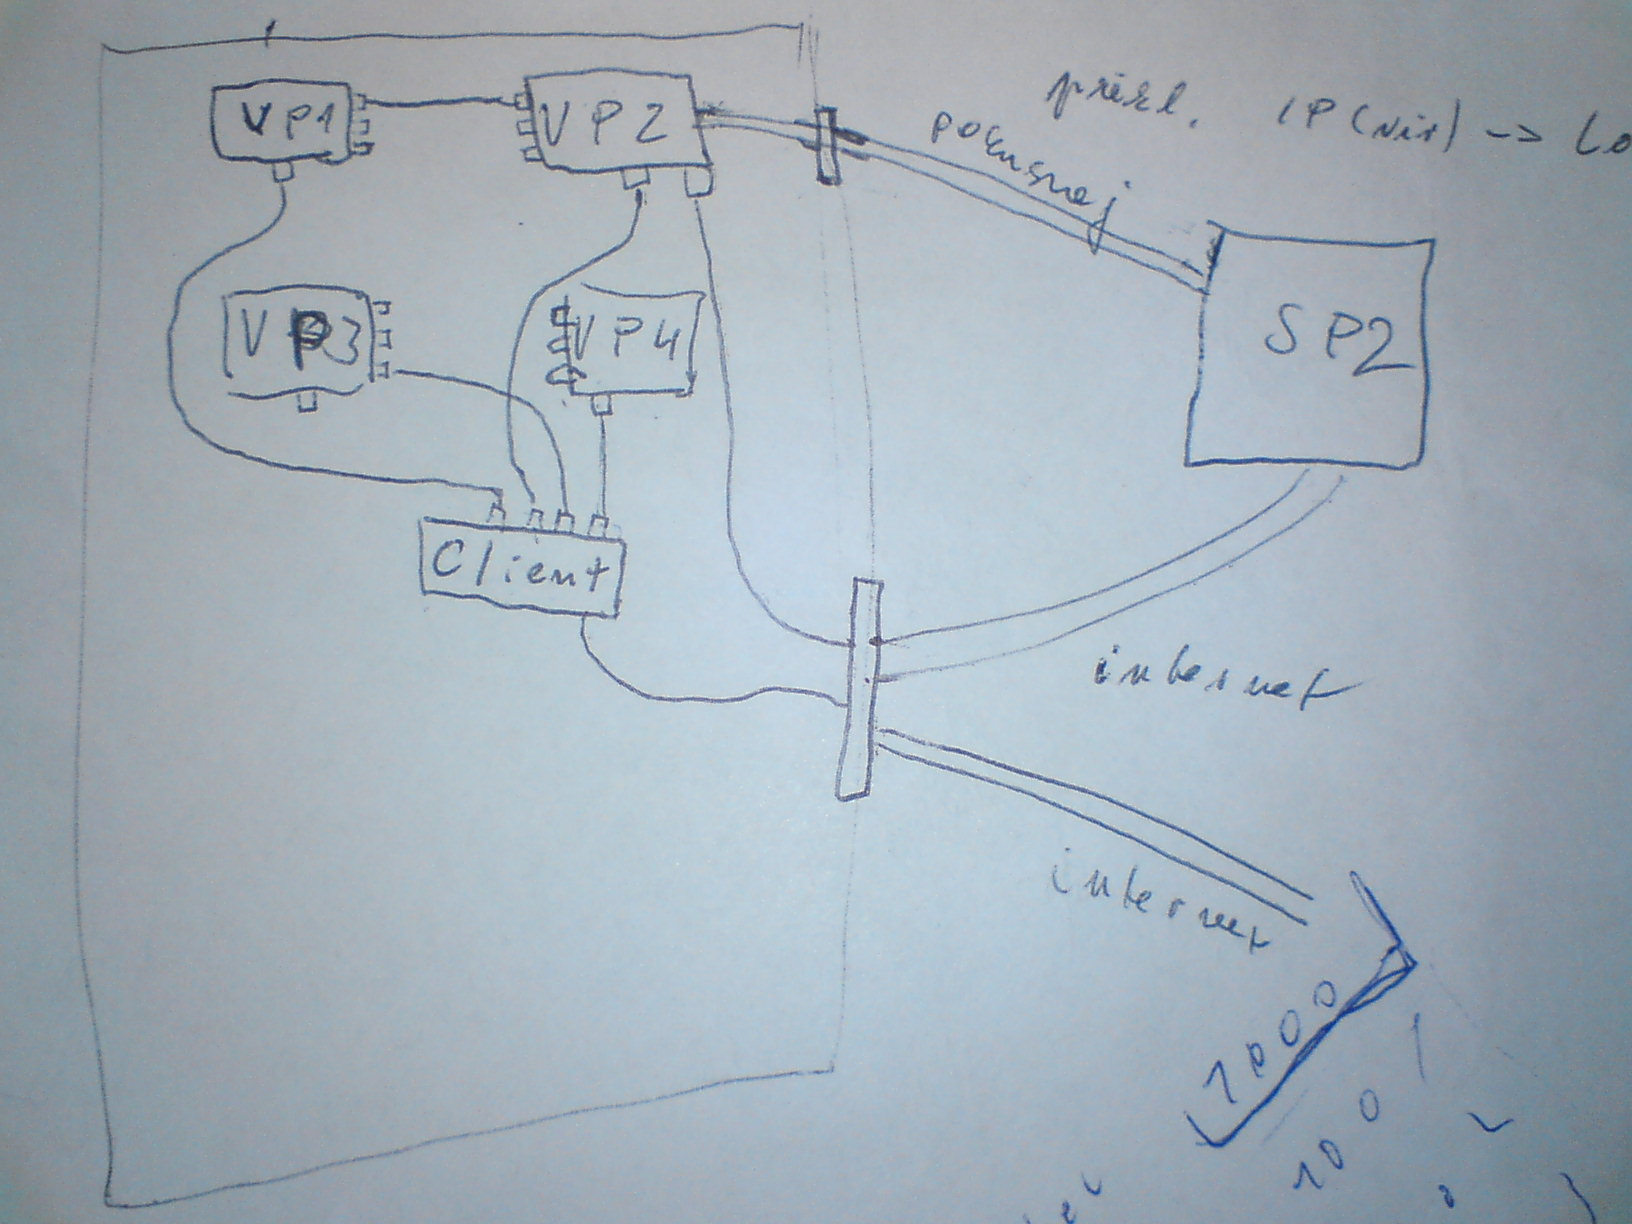
\includegraphics[width=12cm]{figures/navrh}
\caption{Počáteční návrh}
\label{fig:navrh}
\end{center}
\end{figure}

%------------------------------------------------------------------------------

\subsection{Klient - server}\label{klient_server}
Dle nového návrhu bude celá aplikace rozdělena na dvě základní vrstvy:
\begin{itemize}
 \item komunikační - bude zajišťovat spojení mezi klientskou a serverovou částí aplikace
 \item aplikační - bude tvořit zbytek systému (směrování, překlad adres, parsery příkazů, ..)
\end{itemize}

\subsubsection{Komunikační vrstva}
Komunikační vrstva bude složena z~architektury klient - server. Tato vrstva bude převzata ze semestrální práce pro předmět \verb|Y36PSI|, kde bylo za úkol mimo jiné implementovat více-vláknový server. V~této převzaté implementaci je server, ke kterému se připojují klienti. Pro každého klienta se vytvoří nové vlákno, takže není problém obsluhovat více klientů zároveň. 

Cílem aplikace je vytvořit simulátor počítačové sítě, ta bude muset být reprezentována objekty, které budou zastupovat jednotlivé počítače. Každý počítač se bude muset chovat jako server, aby se na něj mohlo připojit více klientů najednou. Tak bude splněn jeden z~funkčních požadavků.

Pro připojení klientů bude použit program \verb|telnet|. Více o~návrhu v~kapitole \ref{telnet}. 


\subsubsection{Aplikační vrstva}
Tuto vrstvu bude tvořit především parser příkazů emulující Cisco IOS, směrování paketů, routovací tabulku a překlad adres. Aplikační vrstva bude kvůli větší přehlednosti více rozebrána v~kapitole Realizace \ref{realizace}.

%------------------------------------------------------------------------------

\subsection{Telnet} \label{telnet}
V~zadání je přímo zmíněno použití programu telnet pro připojení klientů k~serveru. Telnet je ale také protokol, po kterém se domlouvá telnet klient a telnet server. Česká wikipedie píše o~telnet protokolu: \uv{\textit{Protokol přenáší osmibitové znaky oběma směry (duplexní spojení) a je velmi jednoduchý.}}\cite{wiki:telnet} Protokol tedy vše posílá po znaku a protistrana po znaku vše potvrzuje. Telnet protokol začne při navazování spojení vyjednávácí proces, který vyjedná s protistranou budoucí nastavení.

Samotný telnet (ať protokol či program) ale neposkytuje doplňování příkazů nebo alespoň historii příkazů. Dalším problémem je, že při psaní příkazů přes telnet nefunguje editace aktuálního řádku, respektive lze mazat po znacích klávesou \verb|BackSpace|, ale nelze se pohybovat do stran šipkami doleva a doprava - při takovém pokusu to vypíše \verb|^[[D| či \verb|^[[C|. 

Řešením by mohlo být zkusit posílat nějaké speciální znaky pro posun kurzoru do stran, aby server věděl, že má nastat posun vlevo či vpravo. Pak by si musel server pamatovat, na které pozici řádku je klient. Nepřišel jsem však na způsob, jak přesvědčit program telnet pro posílání nějakého znaku na událost \uv{šipka doprava}, takže tento návrh jsem musel zavrhnout.

Posun kurzoru se ale neprojevuje při připojování na vlastní telnet server. To je způsobeno tím, že v~takovém případě se o~editaci řádku a historii příkazů stará samotný server - v~mém případě telnet server a BASH\footnote{Bourne again shell - nejpoužívanější unixový shell}. V~této aplikaci toho ale nelze využít, takže musí být tyto funkcionality na straně klienta, který je bude zajišťovat. 

Pro linux jsem našel program rlwrap (readline wrapper), který přidává všechny tyto užitečné funkce: editace řádky, historie příkazů, doplňování příkazů, obarvení promptu. Pro Windows jsem nic takového nenašel, takže uživatelé OS Windows budou muset tuto aplikaci spouštět přes program Cygwin. Výhodou tohoto řešení je lepší uživatelský komfort linuxové příkazové řádky než nativní Windows konzole \verb|cmd|.

%------------------------------------------------------------------------------

\subsection{Konfigurační soubor}
Při startu serveru by se měla načíst konfigurace ze souboru a měla by být možnost uložit aktuální konfiguraci zpět do stejného souboru. Diskuze nad možnými řešeními je popsána v~kapitole \ref{xml_soubor}.

%------------------------------------------------------------------------------

\subsection{Směrovač}
Na skutečné počítačové síti jsou síťové prvky několika druhů (router, switch, bridge, repeater, ..), ale na laboratorních cvičeních předmětu Y36PSI se  nastavují pouze směrovače ze 3. vrstvy\footnote{Tato \uv{síťová vrstva} se stará o~směrování v~síti a síťové adresování. Dále poskytuje spojení mezi vzdálenými sítěmi, které spolu přímo nesousedí.} síťového ISO/OSI modelu. Proto tato práce bude implementovat pouze jeden typ síťového prvku - směrovač (router). 

%------------------------------------------------------------------------------

\section{Podobnost simulátoru se skutečným směrovačem}\label{kap:podobnost}
Jedním z~cílů projektu je vytvořit systém, který bude co nejvíce podobný skutečnému směrovači cisco. Bude ale potřeba položit někde hranici mezi složitostí a věrností výsledné práce, protože tyto dvě metriky jsou vzájemném protikladu. Cisco IOS je natolik robustní a propracovaný systém, že je v~mých silách implementace pouze úzké části systému, která je nutně potřeba pro splnění cíle. Pravděpodobně budu nucen místy ustoupit a nechat vypsat hlášení, že to či ono není v~mé implementaci podporováno. 

V~samotném parseru příkazů pro Cisco IOS nebude takovéto hlášení téměř vůbec řešeno, protože by to znamenalo implementaci několika stovek pravidel pro všechny příkazy - např. příkaz \verb|ip| má 103 možností v~konfiguračním stavu. Aby ale uživatel měl alespoň nějakou možnost se dopátrat, co je či není podporováno, tak bude přidán příkaz \verb|help| (\verb|help_en| pro výpis v~angličtině), který bude popisovat, jaký příkaz lze v~kterém stavu Cisca použít.

%------------------------------------------------------------------------------

\section{Předpokládaný rozsah}
Celý projekt by měl být v~rozsahu zhruba 10000 řádků kódu. Nejrozsáhlejší třídy budou pravděpodobně datové struktury pro všechny objekty, které budou emulovat skutečné počítače s~rozhraními, routovací a NAT tabulku atd.

%------------------------------------------------------------------------------

\section{Programovací jazyk a prostředí}
Pro implementaci simulátoru jsem si zvolil programovací jazyk Java hned z~několika důvodů. Jazyk je to velmi robustní s~bohatou sadou různých knihoven. Navíc programy vytvořené v~tomto jazyce jsou zpravidla jednoduše přenositelné mezi různými operačními systémy, což je jeden z~bodů nefunkčních požadavků. Jazyk Java disponuje propracovaným systémem výjimek, takže při nějaké neočekávané chybě se dozvím víc, než v~jazyce C++ s~jeho \verb|Segmentation fault|. Neméně významným důvodem je i skutečnost, že s~Javou mám zatím největší zkušenosti.

Celá práce bude implementována v~Netbeans IDE\footnote{Integrated Development Environment} verze 6.8.

%------------------------------------------------------------------------------

\section{Paměťová náročnost}
Paměťová náročnost bude pravděpodobně vyšší než při použití jazyka C++, jelikož javovský garbage collector není úplně ideálním řešením pro uvolňování paměti. Nicméně se neočekává použití tohoto simulátoru pro více než pár desítek virtuálních počítačů, takže spotřeba paměti by neměla překročit požadavky pro běžné aplikace v~Javě. Zaplnění paměti touto aplikací by mohlo být kolem odhadem 10-30MB (+ načtené prostředí JRE).

%------------------------------------------------------------------------------

\section{Uživatelské rozhraní}
Uživatelské rozhraní by mělo být v~zásadě velmi jednoduché. Vše bude ovládáno přes příkazovou řádku, tak jako na skutečném ciscu. Spuštění serveru bude ulehčeno pomocným skriptem \verb|start_server.sh|, který bude zároveň obsahovat nápovědu. Pro připojování klientů budou rovněž připraveny skripty. 

Na obrázku \ref{fig:uziv_rozh} je příklad, jak by mohlo uživatelské rozhraní vypadat pod operačním systémem Linux.

\begin{figure}[h]
\begin{center}
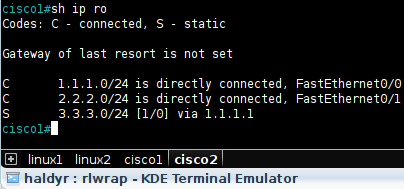
\includegraphics[height=3cm]{figures/uziv_rozhrani}
\caption{Textové rozhraní pro konfiguraci cisca}
\label{fig:uziv_rozh}
\end{center}
\end{figure}









